\documentclass{article}

\usepackage{enumerate}
\usepackage{amsmath,amsthm,amssymb}
\usepackage{tikz}
\usepackage{pgfplots}
\usepackage{multicol}
%\pgfplotsset{compat=newest}

\usepackage[margin=0.5in]{geometry}

\begin{document}

\noindent \textbf{Name:}\underline{\hspace{2in}} \hfill \textbf{Quiz November 6}
\\ \\

\begin{enumerate}
\item (2 points) Answer the following True or False questions. Write out the entire word; if I can't read it, I can't grade it.
  \begin{enumerate}
    \setlength\itemsep{2em}
  \item \underline{\hspace{1in}} A reference angle is always acute.
  \item \underline{\hspace{1in}} The Pythagorean Theorem $a^2 + b^2 = c^2$ is true for every triangle.
  \end{enumerate}
  \vspace{0.2in}
\item (4 points) I am running toward the Eiffel Tower, which I know is 324m tall. When I start running, the angle of inclination between myself and the tower is $5.8^\circ$. After running for 10 minutes, the angle of inclination has increased to $10.2^\circ$.
  \begin{enumerate}
  \item Draw a picture that shows me, the Eiffel Tower, and any relevant distances and angles.
    \vspace{2in}
  \item Use your answer to part (a) to draw two relevant right triangles, with any known side lengths and angle measures labeled.
    \vspace{2in}
  \item How far did I run? (Hint: How far away was I initially, and how far away was I after running?)
    \vspace{1.5in}
  \end{enumerate}
  \vfill
  \hfill (More on the back)
  \newpage
\item (4 points) There's an angle $\theta$, and I don't know what it is. I know that $\tan(\theta) = - 34$ and $\cos(\theta) < 0$.
  \begin{enumerate}
  \item What quadrant does the terminal side of $\theta$ lie in?
    \vspace{0.5in}
  \item Roughly sketch where $\theta$ lies (just getting the quadrant right is enough), and clearly label the reference angle $\theta_R$.
    \begin{center}
      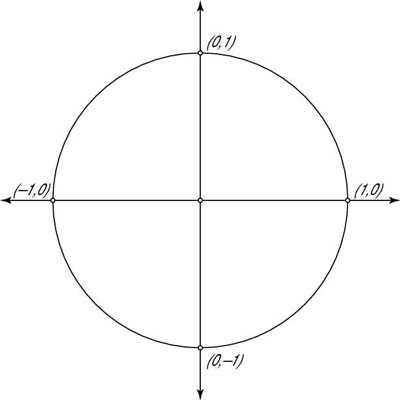
\includegraphics[scale=0.5]{circle.jpg}
    \end{center}
  \item Evaluate all trig functions of $\theta$:
    \begin{multicols}{2}
      $\sin(\theta)=$
      \\ \\ \\ \\
      $\cos(\theta)=$
      \\ \\ \\ \\
      $\tan(\theta)=$
      \\
      $\csc(\theta)=$
      \\ \\ \\ \\
      $\sec(\theta)=$
      \\ \\ \\ \\
      $\cot(\theta)=$
    \end{multicols}
  \end{enumerate}
  \vspace{1.5in}

\end{enumerate}

\end{document}
